\documentclass[a4paper,8pt]{article}
\usepackage[utf8x]{inputenc}
\usepackage{graphicx}
\usepackage{listings}
%opening
\title{Teoría de Lenguajes\\ \textbf{TP2: “Micro HTML Prettyprint - segunda parte”}}
\author{1º Cuatrimestre 2013} 
\date{}


\begin{document}

\maketitle

\begin{center}
\vspace{10cm}

\begin{tabular}{|c|c|}
\hline
\hline
\textbf{Nombre}&\textbf{email}\\
\hline
\hline
Pablo Herrero (LU:332/07)   & pablodherrero@gmail.com   \\
\hline
\hline
\end{tabular}
\end{center}

\newpage

\begin{section}{Introducción}
Como se describe en el enunciado, HTML es un lenguaje de marcado utilizado en la mayoría del contenido de la World Wide Web.
Muchos de los tags que conforman HTML son interpretados por los browsers para permitir la visualización de contenido de manera amigable (human readable). 

Se pide realizar un parser que interprete la estructura de los archivos HTML y que genere otro documento HTML que permita visualizar el HTML original de manera elegante (Prettyprint). Ciertos tags se verán de manera anidada mediante la indentación y los comentarios, tags, atributos y otros elementos de control se verán con diferentes colores (ver ejemplo en la figura 1).

\begin{figure}[h!]
  \centering
  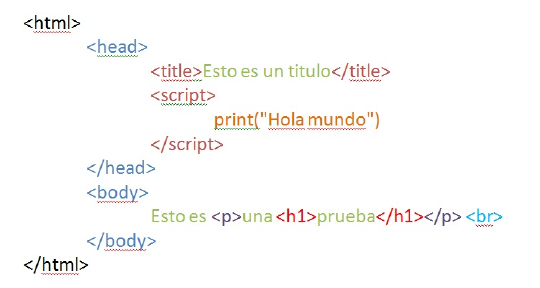
\includegraphics[scale=0.70]{salida.png}
  \caption{\texttt{Salida esperada para el siguiente HTML ``$<html> <head><title>$Esto es un titulo$</title> <!–$ esto es un comentario $–> <script> print($”Hola mundo”$)</script></head> <body>$ Esto es $<p>$una $<h1>$prueba$</h1></p> <br></body></html>$''}}
\end{figure}

El trabajo práctico fue dividido en dos partes, la primera consistió en identificar cuál seria la gramática y los componentes léxicos de nuestro lenguaje y la segunda parte consiste en realizar el parser junto con las reglas semánticas que permitirán generar el HTML resultante.
 


\end{section}
\newpage
\begin{section}{Gramática}
\begin{subsection}{Descripción del HTML reducido a identificar}
Para simplificar el lenguaje, ya que HTML es muy completo y extenso, sólo se considerará un subconjunto de tags válidos, no se permitirán atributos y se espera que todos los tags tengan su tag de cierre correspondiente (salvo $<br>$).\\


Los tags que se considerarán son:

\textbf{$<html>-<head>-<body>-<title>-<script>-<div>-<h1>-<p>-<br>$}.\\

Con las siguiente restricciones:

\begin{itemize}
 \item Es obligatorio que el documento completo esté rodeado por tags de apertura y cierre $<html>$
\item dentro del html puede tener una sección opcional $<head>$ y otra sección también opcional $<body>$. Si hay una sección $<head>$ esta debe encontrarse antes del body.
\item dentro de la sección head pueden aparecer indistintamente y en orden no preestablecido secciones $<title>$ y $<script>$
\item $<title>$ contiene texto sin tags
\item dentro de la sección $<script>$ puede haber cualquier cosa salvo el tag de cierre de dicha sección
\item dentro de la sección $<body>$ tendremos bloques de texto con subsecciones (div, h1 o p) o con tags $<br>$ sueltos, las subsecciones se comportan como la sección $<body>$
\end{itemize}


\end{subsection}

\begin{subsection}{Gramática utilizada para la primera parte del tp}
\bigskip

\begin{verbatim}
S -> E<html>EAE</html>E | E<html>ECE</html>E | E<html>E</html>E
A -> <head>EBE</head>ECE
B -> <title>T</title>EBE | <script>T</script>EBE | lambda
C -> <body>EDE</body> | <body>TDT</body>  | lambda
D -> T D | lambda | <div>EDE</div>EDE | <p>EDE</p> EDE | <h1>EDE</h1> EDE |
    |<br>EDE | <div>TDT</div>TDT | <p>TDT</p>TDT | <h1>TDT</h1>TDT | <br>TDT
E -> espacioE | E<!–-T-–>E  | lambda 
T -> (a|...|z|A|...|Z|0|...|9|...|&|;|espacio|... )T | E |lambda  
espacio pertenece a {“ “}

\end{verbatim}
\bigskip

Descripción de la gramática
\begin{enumerate}
 \item Todas las derivaciones del símbolo distinguido comienzan (terminan) con cero o más espacios y luego un tag de apertura (cierre) de html, la derivación que contiene A corresponde a un HTML con head mientras que la que contiene C es un HTML que no tiene head
 \item La derivación de A corresponde a un head seguido de cero o más espacios, cero o un body y cero o más espacios
\item La derivación de B es el contenido que puede estar dentro de un head, estos son titles (conteniendo texto) o scripts (conteniendo texto), en ambos casos puede haber cero o más ocurrencias
\item La derivación de C permite que haya cero o un body conteniendo tags, ver EDE y TDT en el punto siguiente.
\item Derivaciones de D: a) TD  , esto permite agregar texto a izquierda de los tags, como el tag puede derivar en $\lambda$ esto también permite terminar con texto a derecha “quitando” el último D - b) Las derivaciones rodeades de div, p y h1 permiten generar estos tags, en todos los casos contienen EDE que permite nuevos tags rodeados de cero o más espacios o derivar D a TD y generar texto - c) La derivación $<br>EDE$ permite generar el tag $<br>$ - d) Las derivaciones que contienen TDT son todas redundantes por lo expuesto en 5.a y 5.b pero hacen que los ejemplos sean más compactos
\item Esta derivación permite generar cero o más espacios o comentarios
\item Esta derivación permite generar texto de longitud cero o mayor, se agregan los símbolos $\&$ y $;$ para poder codificar las entidades html y se permite derivar a E para poder incluir comentarios ya que esto siempre es válido
\end{enumerate}

\end{subsection}

\begin{subsection}{Gramática corregida}
En las correcciones se nos indicó que debíamos completar los tokens léxicos para los tags y definir correctamente el conjunto de terminales para el texto.
\bigskip

\begin{verbatim}
S -> E I_HTML EAE F_HTML E | E I_HTML ECE F_HTML E | E I_HTML E F_HTML E
A -> I_HTML EBE F_HTML ECE
B -> I_TITLE T F_TITLE EBE | I_SCRIPT T F_SCRIPT EBE | lambda
C -> I_BODY EDE F_BODY | I_BODY TDT F_BODY  | lambda
D -> T D | lambda | I_DIV EDE F_DIV EDE | I_P EDE F_P EDE | 
     | I_H1 EDE F_H1 EDE | I_BR EDE | I_DIV TDT F_DIV TDT | 
     | I_P TDT F_P TDT | I_H1 TDT F_H1 TDT | I_BR TDT
E -> WS E | E I_COMMENT T F_COMMENT E  | lambda 
T -> WS TEXTO_SIN_TAGS WS T | lambda 

---------------- TOKENS LEXICOS ---------------------------
I_HTML 	:	'<html>' 
F_HTML 	:	'</html>' 

I_HEAD 	:	'<head>'  
F_HEAD 	:	'</head>' 

I_BODY 	:	'<body>' 
F_BODY 	:	'</body>'

I_TITLE:	'<title>'  
F_TITLE:	'</title>' 
	
I_SCRIPT:	'<script>'  
F_SCRIPT:	'</script>' 
	
I_DIV 	:	'<div>' 
F_DIV 	:	'</div>' 
	
I_H1 	:	'<h1>'  
F_H1 	:	'</h1>' 
	
I_P 	:	'<p>'
F_P 	:	'</p>' 

BR 	:	'<br>'

I_COMMENT:	'<!–-'
F_COMMENT:	'-->'

TEXTO_SIN_TAGS 
	:	(~('<' | '>' | '\t' | '\r'| '\n'))* 

WS 
    :   ('\t' | '\r'| '\n') 


\end{verbatim}
\bigskip
\newpage
 \begin{subsubsection}{Arboles de derivación - Ejemplos}
       \begin{figure}[h!]
      \centering
      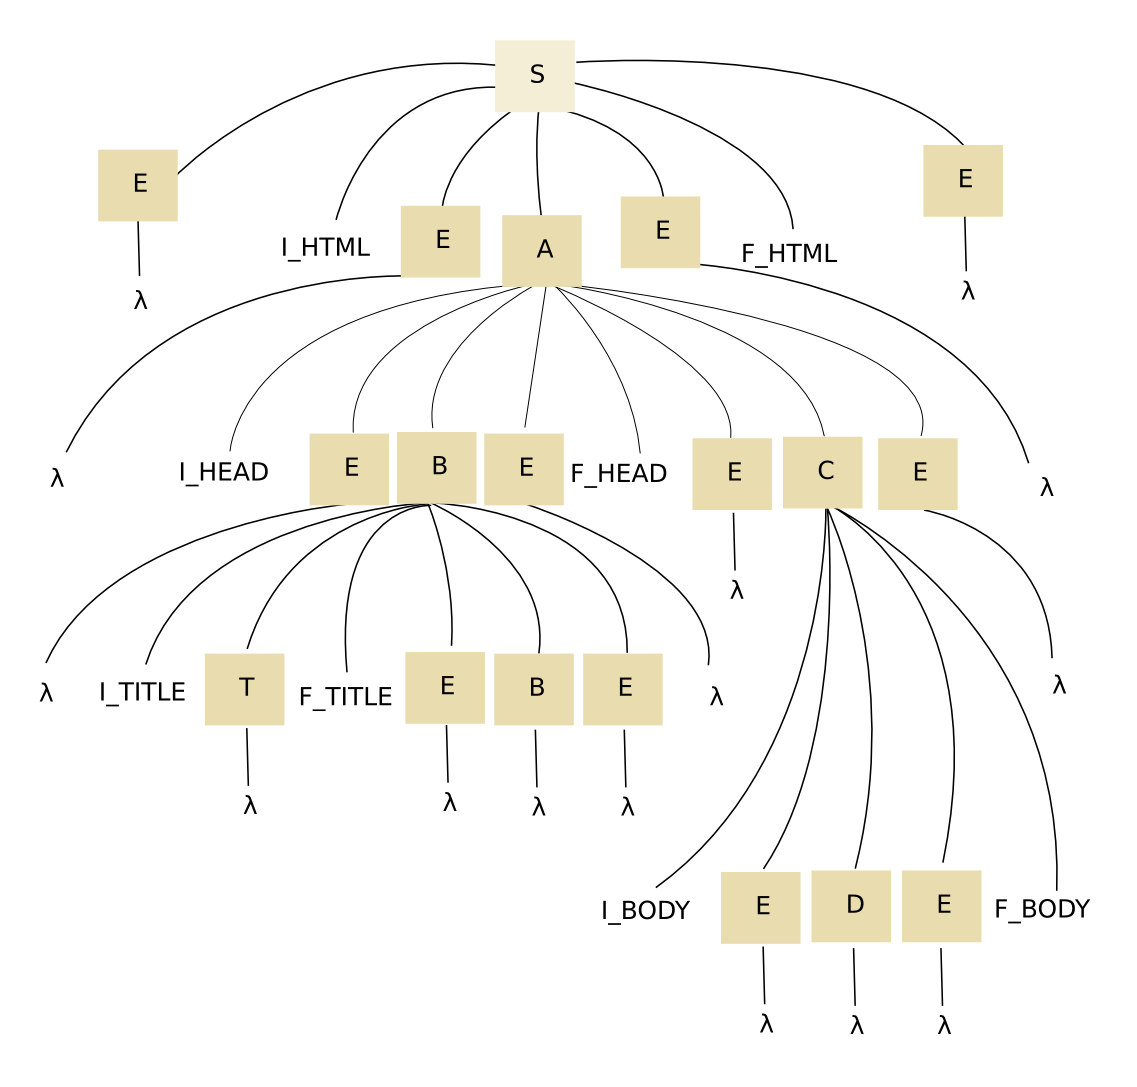
\includegraphics[scale=0.30]{ejemplo1.png}

      \caption{Arbol de derivación para ``$<html><head><title></title></head><body></body></html>$''}
    \end{figure}

    \begin{figure}[h!]
      \centering
      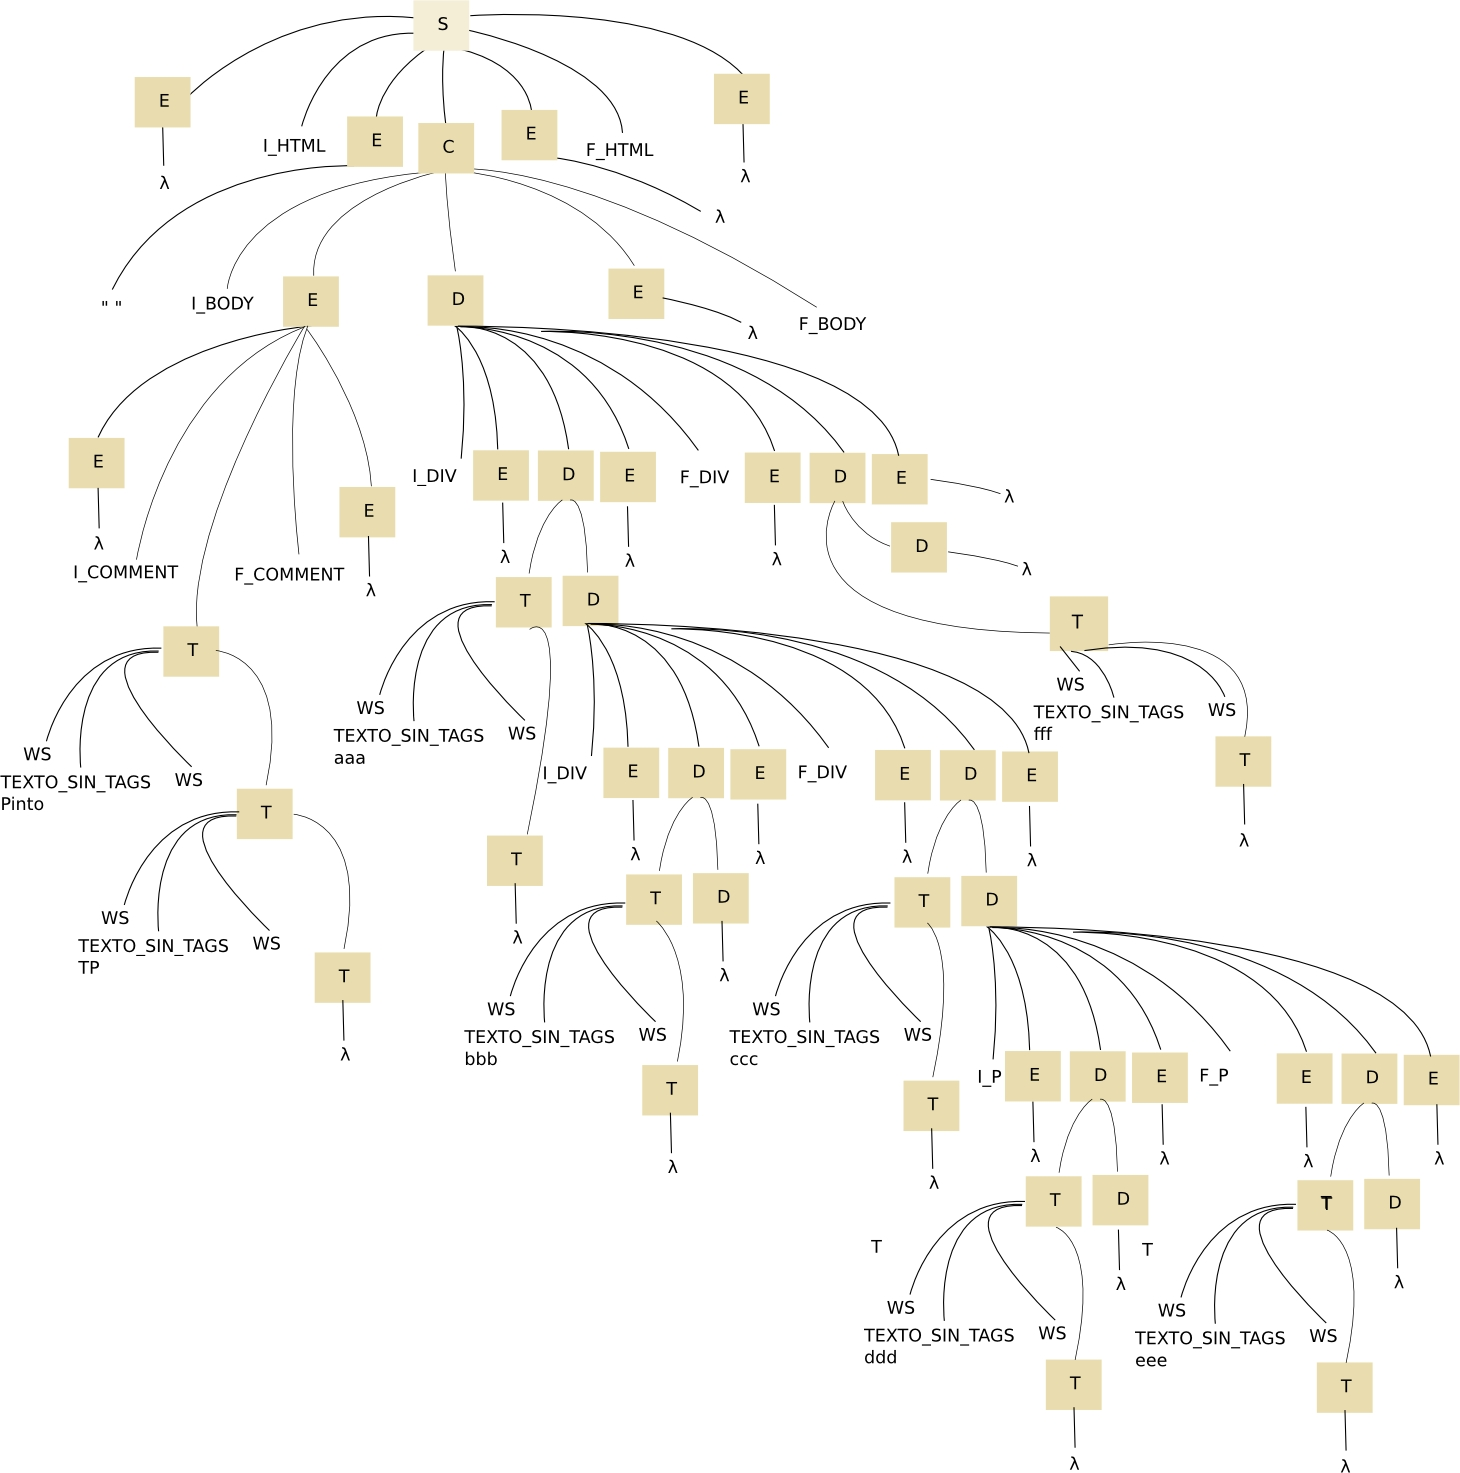
\includegraphics[scale=0.35]{g5188.jpg}

      \caption{Arbol de derivación para ``$<html> <body><!--$ pinto TP $--> <div>aaa<div>bbb</div>ccc<p>ddd</p>eee</div>fff</body></html>$''}
    \end{figure}


 \end{subsubsection}

\end{subsection}
\newpage

\begin{subsection}{Gramática modificada para la segunda parte del tp}

Tomando como base las correciones a la gramática entregada en la primera parte se optó por reescribir la gramática desde el comienzo.\\

En esta segunda parte, una vez definida la gramática, se agregarán en la implementación reglas semánticas que permitan:\\
\begin{itemize}
 \item La salida será un documento que se visualice desde un browser como código HTML (Figura 1).
\item El código del HTML de entrada deberá aparecer formateado con cada línea indentada según el nivel de anidación del código del archivo HTML de origen. 
\item A cada clase de token se le deben poder asignar distintos atributos visuales. En cuanto a los atributos visuales, se requiere un color para los tags head y body, otro para los tags title y script, otro para el tag h1, otro para el tag div y otro para el tag br. Otro color para el texto y otro para los scripts.
Se sugiere que cada token quede incluido en un elemento de tipo SPAN que indique de qué clase es.
Por ejemplo:$<SPAN class=``tagH1''>\&lt;h1\&gt;</SPAN>.$

\end{itemize}
Agregamos como restricción que dentro de los comentarios no permitimos '-' ya que se usan para indentificar el cierre simplificando la gramática, a pesar que nos indicaron que se puede negar una cadena usando $~('-->')$ esto no funcionó o no lo pudimos hacer funcionar.

Luego de evaluar las diferentes herramientas de generación de código a partir de gramáticas y de elegir AntLR quedó definido el tipo de gramática que debíamos utilizar, esta sería ELL(1) ya que es la soportada por la herramienta.
Nuestro objetivo fue, desde el comienzo, dar a la gramática todo el poder posible para luego escribir la menor cantidad de código, creemos que logramos este objetivo (ver sección 3.4).

\bigskip

\begin{verbatim}
  
//------------------ GRAMATICA -----------------------------
html 	:	ws* I_HTML head? body? ocultar F_HTML;

head 	:	ocultar I_HEAD (ws | COMENTARIO | title | script)* F_HEAD;

title 	:	I_TITLE texto_o_comentarios F_TITLE;
script 	:	I_SCRIPT texto_o_comentarios F_SCRIPT;

body 	:	ocultar I_BODY tags F_BODY;

tags	:	texto_o_comentarios tag*;

tag	:	(I_DIV tags F_DIV | I_H1 tags F_H1 | I_P tags F_P | BR) texto_o_comentarios;

ocultar	:	(ws | COMENTARIO)*;

texto_o_comentarios
	:	(COMENTARIO | TEXTO_SIN_TAGS)*;

ws 
    :   ('\t' | '\r'| '\n' | ' ')
    ;

//---------------- TOKENS LEXICOS ---------------------------
I_HTML 	:	'<html>' ;
F_HTML 	:	'</html>';

I_HEAD 	:	'<head>'  ;
F_HEAD 	:	'</head>' ;

I_BODY 	:	'<body>' ;
F_BODY 	:	'</body>' ;

I_TITLE
 	:	'<title>'  ;
F_TITLE 
	:	'</title>' ;
	
I_SCRIPT
 	:	'<script>'  ;
F_SCRIPT 
	:	'</script>' ;
	
I_DIV 	:	'<div>'  ;
F_DIV 	:	'</div>' ;
	
I_H1 	:	'<h1>' ;
F_H1 	:	'</h1>' ;
	
I_P 	:	'<p>'  ;
F_P 	:	'</p>' ;

BR 	:	'<br>' ;

COMENTARIO 
	:	'<!--' (~('-'))* '-->';

TEXTO_SIN_TAGS 
	:	(~('<' | '>' | '\t' | '\r'| '\n'))+ ;


 \end{verbatim} 



\end{subsection}
\end{section}
\newpage

\begin{section}{Implementación}
\begin{subsection}{Discusión}
%Descripción y decisiones tomadas
En cuanto al lenguaje a utilizar para la implementación evaluamos por separado distintas posibilidades:
\begin{itemize}
 \item Utilizar ANTLR junto con Eclipse en un entorno GNU agregando la semántica en java.
\item Utilizar Ruby
\item Utilizar .NET en un entorno Windows
\end{itemize}

No encontramos consenso en un tiempo razonable. Finalmente se muestran los resultados de la implementación realizada en .NET.\\

Es interesante notar que aunque en toda la documentación y los foros se indica que .Net es compatible encontramos numerosos obstáculos a la hora de integrar la herramienta y el lenguaje, esperamos que el conocimiento adquirido al hacer este TP pueda servir a otros en el futuro, esta es la combinación de herramientas y entornos que finalmente se utilizó:
\begin{itemize}
 \item Visual Studio 2012
\item antlrworks-1.4
\item AntLR 3
\item DOT-NET-runtime-3.1.3 (de AntLR)
\item options { language = 'CSharp2'; output=AST; } en la gramática
\end{itemize}


Uno de los inconvenientes encontrados al escribir la gramática fue que una gramática válida generaba un parser que se "colgaba" con inputs inválidos, para determinar que pasaba debuggeamos el código fuente de AntLR y encontramos un bug que produce esto cuando un token deriva en lambda, el parser generado lo encola una y otra vez en un while infinito intentando parsear el input inválido, el corte se produce por una Exception de OutOfMemory, la solución es que ningún TOKEN derive en lambda, si es necesario se lo convierte en una regla semántica (como bien se dijo en clase el límite entre léxico y semántico en AntLR es bastante difuso) .

Finalmente no pudimos utilizar el channel=Hidden y otras facilidades del AntLRWorks por varias razones:
\begin{enumerate}
 \item Si intentábamos ocultar el espacio entre tags teníamos problemas con los espacios entre palabas (que no queríamos ocultar)
\item Solo se pueden negar caracteres por lo que no se puede identificar algo que no sea $<!-- ......... -->$  de forma sencilla y ocultarlo
\item La forma "greedy" en la que funciona el parser generado hace que al matchear un TOKEN se busque la expresión correspondiente y se trabaja a partir de ahí, esto quiere decir que un comentario dentro de un $<html>$ $</html>$ será matcheado en primer lugar dentro de la derivación que genera estos tags y luego no se matcheará el comentario como un TOKEN a ignorar. Esto, seguramente, es por un error nuestro en el uso de la herramienta; aunque hicimos innumerables pruebas tratando de resolverlo para poder usar el channel=HIDDEN no tuvimos éxito y tuvimos que modificar la gramática para matchear comentarios y caracteres vacíos y luego ignorarlos, vale aclarar que el resultado final es el mismo.

\end{enumerate}


\end{subsection}
\newpage
\begin{subsection}{Resultados}
\begin{tabular}{|p{6.5cm}|p{6.5cm}|}
\hline 
\multicolumn{2}{|c|}{Ejemplo 1}\\
\hline 
\textbf{Input}&\textbf{Output}\\
\hline 
 \footnotesize{\begin{verbatim}<html><head><title></title></head>
<body></body></html>\end{verbatim}}

\bigskip
\textbf{Browser}\linebreak \linebreak
\centering 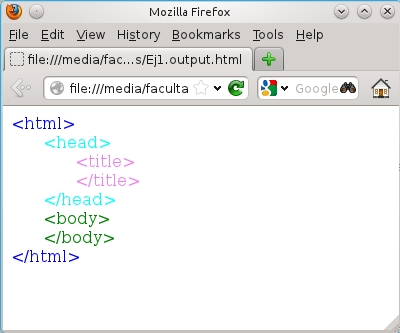
\includegraphics[scale=0.50]{ej1_out.jpg} & \footnotesize{\begin{verbatim}<html>
    <head>
        <style TYPE='text/css'>
            SPAN { display: block; }
            DIV.bloque { margin-left: 2em; }
            SPAN.tagScript { color: orange; }
            SPAN.tagP { color: fuchsia; }
            SPAN.tagH1 { color : brown; }
            SPAN.tagDiv { color : red; }
            SPAN.tagHtml { color : blue; }
            SPAN.tagBody { color : green; }
            SPAN.tagHead { color : cyan; }
            SPAN.tagTitle { color : violet; }
            SPAN.tagBr { color : yellow; }
        </style>
    </head>
    <body>
<span class='tagHtml'>&lt;html&gt;</span>
<div class='bloque'>
<span class='tagHead'>&lt;head&gt;</span>
<div class='bloque'>
<span class='tagTitle'>&lt;title&gt;</span>
<div class='bloque'>
</div>
<span class='tagTitle'>&lt;/title&gt;</span>
</div>
<span class='tagHead'>&lt;/head&gt;</span>
<span class='tagBody'>&lt;body&gt;</span>
<div class='bloque'>
</div>
<span class='tagBody'>&lt;/body&gt;</span>
</div>
<span class='tagHtml'>&lt;/html&gt;</span>

    </body>
</html>\end{verbatim}}\\
\hline

\end{tabular}


\begin{tabular}{|p{6.5cm}|p{6.5cm}|}
\hline 
\multicolumn{2}{|c|}{Ejemplo 4}\\
\hline 
\textbf{Input}&\textbf{Output}\\
\hline
 \footnotesize{\begin{verbatim} <html>
<head>
<title>Este es un gran TP</title>
</head>
<body>
Aca comienza el body.
Ahora pongamos un div!
<div>estoy adentro de un div</div>
termino el div, pongamos un p
<p>
este es un parrafo genial
</p>
y listo, terminamos
</body>
</html>\end{verbatim}}  
\bigskip
\textbf{Browser}\linebreak \linebreak
\centering 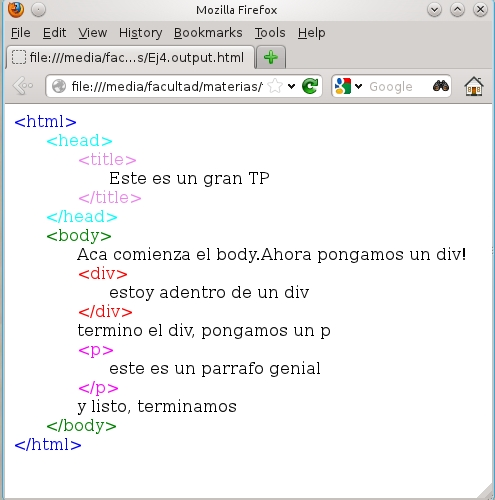
\includegraphics[scale=0.50]{ej4_out.jpg} & \footnotesize{\begin{verbatim}<html>
    <head>
        <style TYPE='text/css'>
            SPAN { display: block; }
            DIV.bloque { margin-left: 2em; }
            SPAN.tagScript { color: orange; }
            SPAN.tagP { color: fuchsia; }
            SPAN.tagH1 { color : brown; }
            SPAN.tagDiv { color : red; }
            SPAN.tagHtml { color : blue; }
            SPAN.tagBody { color : green; }
            SPAN.tagHead { color : cyan; }
            SPAN.tagTitle { color : violet; }
            SPAN.tagBr { color : yellow; }
        </style>
    </head>
    <body>
<span class='tagHtml'>&lt;html&gt;</span>
<div class='bloque'>
<span class='tagHead'>&lt;head&gt;</span>
<div class='bloque'>
<span class='tagTitle'>&lt;title&gt;</span>
<div class='bloque'>
Este es un gran TP
</div>
<span class='tagTitle'>&lt;/title&gt;</span>
</div>
<span class='tagHead'>&lt;/head&gt;</span>
<span class='tagBody'>&lt;body&gt;</span>
<div class='bloque'>
Aca comienza el body.Ahora pongamos un div!
<span class='tagDiv'>&lt;div&gt;</span>
<div class='bloque'>
estoy adentro de un div
</div>
<span class='tagDiv'>&lt;/div&gt;</span>
termino el div, pongamos un p
<span class='tagP'>&lt;p&gt;</span>
<div class='bloque'>
este es un parrafo genial
</div>
<span class='tagP'>&lt;/p&gt;</span>
y listo, terminamos
</div>
<span class='tagBody'>&lt;/body&gt;</span>
</div>
<span class='tagHtml'>&lt;/html&gt;</span>

    </body>
</html>\end{verbatim}}\\
\hline

\end{tabular}


\begin{tabular}{|p{6.5cm}|p{6.5cm}|}
\hline 
\multicolumn{2}{|c|}{Ejemplo 6}\\
\hline 
\textbf{Input}&\textbf{Output}\\
\hline 
 \footnotesize{\begin{verbatim}
Error!!
<html>
<head>
<title>Este es un gran TP</title>
</head>
<body>
este es el body de un ejemplo con errores
<div>y tiene un div!!</div>
</body>
</html>                      
\end{verbatim}}
\bigskip

\textbf{Browser}\linebreak \linebreak
\centering 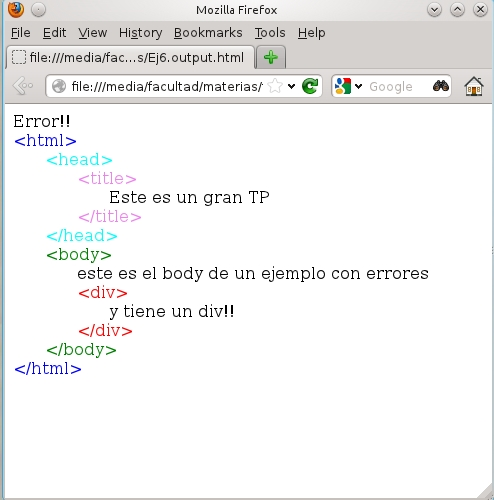
\includegraphics[scale=0.50]{ej6_out.jpg} & \footnotesize{\begin{verbatim}<html>
    <head>
        <style TYPE='text/css'>
            SPAN { display: block; }
            DIV.bloque { margin-left: 2em; }
            SPAN.tagScript { color: orange; }
            SPAN.tagP { color: fuchsia; }
            SPAN.tagH1 { color : brown; }
            SPAN.tagDiv { color : red; }
            SPAN.tagHtml { color : blue; }
            SPAN.tagBody { color : green; }
            SPAN.tagHead { color : cyan; }
            SPAN.tagTitle { color : violet; }
            SPAN.tagBr { color : yellow; }
        </style>
    </head>
    <body>
Error!!
<span class='tagHtml'>&lt;html&gt;</span>
<div class='bloque'>
<span class='tagHead'>&lt;head&gt;</span>
<div class='bloque'>
<span class='tagTitle'>&lt;title&gt;</span>
<div class='bloque'>
Este es un gran TP
</div>
<span class='tagTitle'>&lt;/title&gt;</span>
</div>
<span class='tagHead'>&lt;/head&gt;</span>
<span class='tagBody'>&lt;body&gt;</span>
<div class='bloque'>
este es el body de un ejemplo con errores
<span class='tagDiv'>&lt;div&gt;</span>
<div class='bloque'>
y tiene un div!!
</div>
<span class='tagDiv'>&lt;/div&gt;</span>
</div>
<span class='tagBody'>&lt;/body&gt;</span>
</div>
<span class='tagHtml'>&lt;/html&gt;</span>

    </body>
</html>\end{verbatim}}\\
\hline

\end{tabular}

\end{subsection}
\begin{subsection}{Ejemplos de uso}
El programa es realmente sencillo, recibe por STDIN un HTML (válido o no), devuelve por STDOUT el PreetyPrint (un HTML con estilos embebidos que se puede abrir en cualquier browser) y por STDERROR los errores (de existir) encontrados en el INPUT.
Utilización:\\
\begin{itemize}
 \item Ingresar
  \begin{verbatim}
       TeoriaDeLenguajes.exe < input.html > output.html
  \end{verbatim}

\end{itemize}


\end{subsection}
\begin{subsection}{Código Fuente}
\begin{subsubsection}{TPTLeng.g}
 \begin{verbatim}
using System;
using System.Collections.Generic;
using System.IO;
using System.Linq;
using Antlr.Runtime;

namespace TeoriaDeLenguajes
{
    class Program
    {
        private static readonly Dictionary<String, String> 
                 Traduccion = new Dictionary<String, String>
            {
                {"extraneous input", "entrada extraña"},
                {"expecting", "se esperaba"},
                {"line", "linea"},
                {"mismatched character", "caracter incorrecto"},
                {"mismatched input", "entrada incorrecta"},
                {"no viable alternative", "no existe alternativa valida"},
                {"at character", "en el caracter"},
                {"at input", "en la entrada"}
            };

        private static void Main(string[] args)
        {
            if (args.Length != 0)
            {
                Console.WriteLine();
                Console.WriteLine();
                Console.WriteLine("Ingrese el html, una linea vacia termina la carga
                y comienza el parse, puede redireccionar STDIN y STDOUT");
                
                Console.WriteLine();
                Console.WriteLine("TeoriaDeLenguajes.exe < input.html > output.html");
                Console.WriteLine();
                Console.WriteLine();
                return;
            }
            String entrada = String.Empty;
            String nuevaLinea;
            do
            {
                nuevaLinea = Console.ReadLine();
                entrada += nuevaLinea;
            } while (!String.IsNullOrEmpty(nuevaLinea));

                //" <html> <head><title>Esto es un título</title>
                // <!- esto es un comentario --> <script>print(”Hola mundo”)
                // </script></head> <body> Esto es <p>una <h1>prueba</h1>
                // </p><br></body></html>";

            ANTLRStringStream input = new ANTLRStringStream(entrada);
            TPTLengLexer lexer = new TPTLengLexer(input);

            CommonTokenStream tokens = new CommonTokenStream(lexer);

            TPTLengParser parser = new TPTLengParser(tokens);

            Console.Write(
@"<html>
    <head>
        <style TYPE='text/css'>
            SPAN { display: block; }
            DIV.bloque { margin-left: 2em; }
            SPAN.tagScript { color: orange; }
            SPAN.tagP { color: fuchsia; }
            SPAN.tagH1 { color : brown; }
            SPAN.tagDiv { color : red; }
            SPAN.tagHtml { color : blue; }
            SPAN.tagBody { color : green; }
            SPAN.tagHead { color : cyan; }
            SPAN.tagTitle { color : violet; }
            SPAN.tagBr { color : yellow; }
        </style>
    </head>
    <body>
");
            StringWriter errors = new StringWriter();
            TextWriter standardError = Console.Error;
            Console.SetError(errors);

            parser.html();

            Console.SetError(standardError);

            Console.Error.Write(Traduccion.Aggregate(errors.ToString(),
                (current, traduccion) => current.Replace(traduccion.Key, 
                traduccion.Value)));

            Console.Write(@"
    </body>
</html>");
            //Console.ReadKey();
        }
    }
}





grammar TPTLeng;

options 
{
	language = 'CSharp2';
	output=AST; 
} 
/*
@parser::members {
/*
  public static void main(String[] args) throws Exception {
    String text = args[0];
    ANTLRStringStream in = new ANTLRStringStream(text);
    TestLexer lexer = new TestLexer(in);
    CommonTokenStream tokens = new CommonTokenStream(lexer);
    System.out.println(new TestParser(tokens).mainRule());
  }
*/
/*
protected override Object RecoverFromMismatchedToken(
      IIntStream nuevoInput, int ttype, BitSet follow)
{
	throw new Exception();
	throw new MismatchedTokenException(ttype, nuevoInput);
}

public override Object RecoverFromMismatchedSet(
      IIntStream nuevoInput, RecognitionException e, BitSet follow)
{
	throw new Exception();
	throw e;
}

}

@rulecatch {
    catch (RecognitionException e) {
	throw new Exception();
        throw e;
    }
}

@lexer::members {


public override void Recover(RecognitionException e)
{     throw new Exception();   }

public override void ReportError(RecognitionException e) {
	//throw new RuntimeException(e);
	throw new Exception();
}

} 
*/
/*
@lexer::namespace {
    System
}

@parser::namespace {
    System
}*/

/*
public eval returns [double value]
    :    expr=e {$value = $expr.value;}
    ;

e returns [double value] // additionExp
    :    t2=t        {$value = $t2.value;}
         ( '+' t2=t  {$value += $t2.value;}
         | '-' t2=t  {$value -= $t2.value;} 
         )* 
    ;

t  returns [double value] // multiplyExp
    :    f2=f        {$value = $f2.value;} 
         ( '*' f2=f  {$value *= $f2.value;} 
         | '/' f2=f  {$value /= $f2.value;} 
         )* 
    ;


f returns [double value] // atomExp
    :    n=Numero     {$value = double.Parse($n.text);}
    |    '(' exp=e ')'  {$value = $exp.value;}
    ;
*/
@lexer::members {
private void ImprimirTag(String tag, Boolean? inicio)
{
	if (inicio.HasValue && !inicio.Value) { Console.WriteLine("</div>"); }
	Console.WriteLine("<span class='tag{0}'>&lt;{1}{2}&gt;</span>", 
	  UppercaseFirst(tag), inicio.HasValue && !inicio.Value ? "/" : String.Empty, tag);
	if (inicio.HasValue && inicio.Value) { Console.WriteLine("<div class='bloque'>"); }
}

private static String UppercaseFirst(String s)
{
	return String.IsNullOrEmpty(s) ? String.Empty : Char.ToUpper(s[0]) + s.Substring(1);
}




}
//------------------ GRAMATICA -----------------------------
html 	:	ws* I_HTML head? body? ocultar F_HTML;

head 	:	ocultar I_HEAD (ws | COMENTARIO | title | script)* F_HEAD;

title 	:	I_TITLE TEXTO_SIN_TAGS? F_TITLE;
script 	:	I_SCRIPT TEXTO_SIN_TAGS? F_SCRIPT;

body 	:	ocultar I_BODY tags F_BODY;

tags	:	TEXTO_SIN_TAGS? tag*;

tag	:	(I_DIV tags F_DIV | I_H1 tags F_H1 | I_P tags F_P | BR) TEXTO_SIN_TAGS?;

ocultar	:	(ws | COMENTARIO)*;

ws 
    :   ('\t' | '\r'| '\n' | ' ')
    ;

//---------------- TOKENS LEXICOS ---------------------------
I_HTML 	:	'<html>'  { ImprimirTag("html", true); };
F_HTML 	:	'</html>' { ImprimirTag("html", false); };

I_HEAD 	:	'<head>'  { ImprimirTag("head", true); };
F_HEAD 	:	'</head>' { ImprimirTag("head", false); };

I_BODY 	:	'<body>'  { ImprimirTag("body", true); };
F_BODY 	:	'</body>' { ImprimirTag("body", false); };

I_TITLE
 	:	'<title>'  { ImprimirTag("title", true); };
F_TITLE 
	:	'</title>' { ImprimirTag("title", false); };
	
I_SCRIPT
 	:	'<script>'  { ImprimirTag("script", true); };
F_SCRIPT 
	:	'</script>' { ImprimirTag("script", false); };
	
I_DIV 	:	'<div>'  { ImprimirTag("div", true); };
F_DIV 	:	'</div>' { ImprimirTag("div", false); };
	
I_H1 	:	'<h1>'  { ImprimirTag("h1", true); };
F_H1 	:	'</h1>' { ImprimirTag("h1", false); };
	
I_P 	:	'<p>'  { ImprimirTag("p", true); };
F_P 	:	'</p>' { ImprimirTag("p", false); };

BR 	:	'<br>' { ImprimirTag("br", null); };

COMENTARIO 
	:	'<!--' (~('-'))* '-->';

TEXTO_SIN_TAGS 
	:	(~('<' | '>' | '\t' | '\r'| '\n'))+ { Console.WriteLine(Text); };

 \end{verbatim}

\end{subsubsection}

\end{subsection}
\end{section}
\newpage
\begin{section}{Conclusiones}
Nos pareció muy interesante usar lo aprendido en la materia en una situación cuasi-real.

En cuanto a la implementación, nos parece que lo más importante a destacar de la experiencia fue el tiempo que ahorra la generación de código a partir de gramáticas, no sólo el primer parser lo obtuvimos en un tiempo mucho menor al que nos hubiera tomado escribirlo nosotros sino que su código es mucho más robusto y agregarle funcionalidad requiere mínimo esfuerzo extra. 

Una vez instalado el entorno de trabajo fue muy sencillo generar nuevos parsers y probarlos, el uso de pruebas unitarias nos permitió mejorarlo rápidamente sin riesgo de arruinar funcionalidad existente.

Esperamos poder usar lo aprendido en el futuro.
\end{section}
\newpage

\end{document}
